
\chapter{APPENDIX} \label{ch:table appendix}

%\vspace{-0.2in}

%\section{Description of GOY Shell Model Runs and Table}

%In most cases, we have forced the models in the first shell so that the inertial range %forms on the ultraviolet side.  However, in run 2 from Table \ref{table: app GOY table}, %we force in shell seven and observe an infra-red inertial range form.  Run 1 uses the %parameters of \cite{Yamada} originally used.  This run is used as a control and to %reproduce Pisarenko et. al. \cite{Pisarenko} work.  Run 2 is equivalent to Run 1 as far %as the parameters are concerned.  However, in this run, we force in shell 6.  As a %result, we see an infra-red inertial range.  We can apply the affine collapse to this %data as well. This result is of interest in the light of Carl Gibson idea that the true %cascade in turbulence is from small to large scales \cite{Gibson}. We start with small %forcing in Run 3.  Here, the forcing is small enough that the solution is quasi-periodic %and we have no inertial range.  We can observe this in the distribution of $u_n$.  In %this particular case, the points were located in a ring that was centered at the origin %(see Figure \ref{fig: circ symtrc}).   However, there is still circular symmetry about %the origin in this case.

%\begin{figure}[!htp]
%    \begin{center}
%        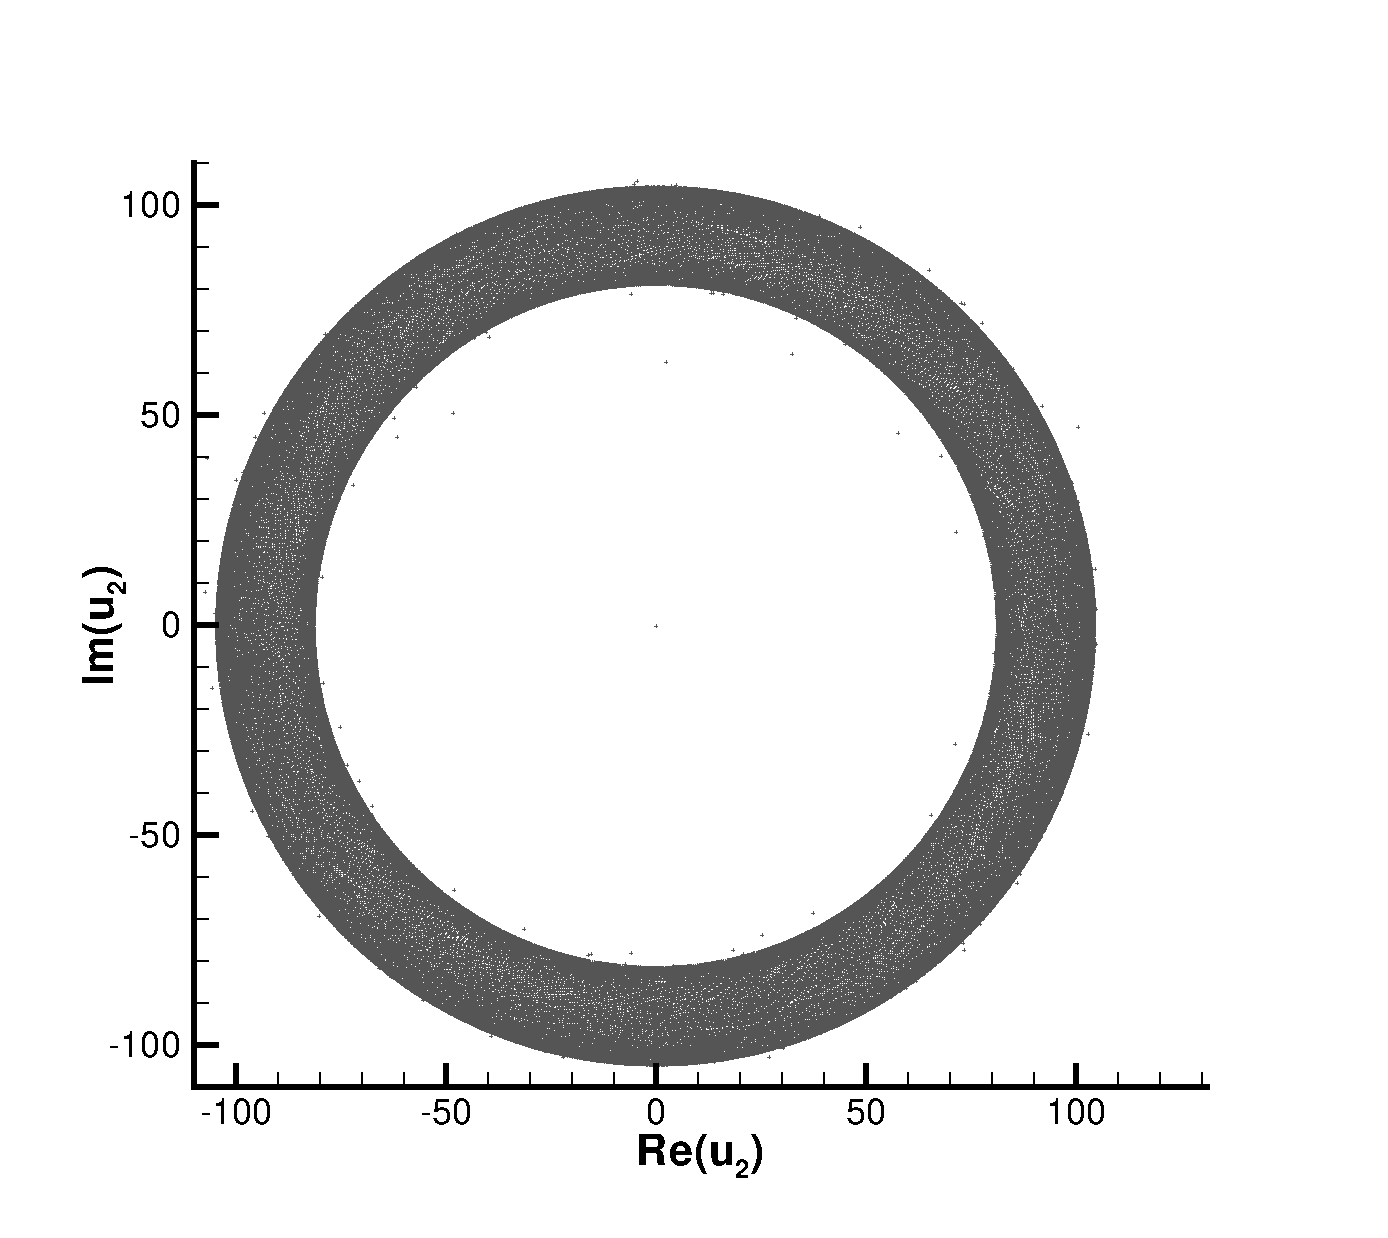
\includegraphics[width=4in]{ns_run10urui.eps}
%    \end{center}
%    \caption{Distribution of $u_i$. This plot displays the quasi-periodic nature of Run 3 %for shell 10 (eps file).} \label{fig: circ symtrc}
%\end{figure}



\section{Meep scripts}

The shell script shown in \autoref{meeptestsh} calls Meep in a loop, increasing the domain size from 128x64 cells (not including PML layers) to 8192x4096 cells in increments of 128x64 cells. 

\lstinputlisting[label=meeptestsh, language=bash,caption=Meep shell script]{meep-test.sh}


The Meep CTL code in \autoref{benchmarkctl} defines a simulation with a dielectric block with $\epsilon_{max}$ = 9. The simulation is run for 5000 frames for each domain size calculated in \autoref{meeptestsh}. During testing, the simulation is timed and the results are written to a CSV file for later analysis. 

\lstinputlisting[label=benchmarkctl,caption={Meep simulation CTL script}]{benchmark.ctl}

\section{GoLightly configuration}

Unlike Meep, GoLightly encodes most simulation parameters in an image file, typically generated in an image editing tool such as Adobe Photoshop or Microsoft Paint. That process is detailed in \autoref{sec:modelProcessor}. 

Additional parameters may be specified on the command line or in a text file. Valid options in the configuration text file are:

\begin{table}[h!]
	\label{golightlyConfig}
	\centering
	\caption{GoLightly Configuration}
	\label{tab:golightlyConfigTerms}
	\begin{tabular}{l | l}
		Option	& Description \\
		\hline
			model     & image file with encoded dielectric, source and monitor properties \\
			nogl      & disable OpenGL visualizer										  \\
			lambda    & source wavelength												  \\
			runlength & number of frames to run the simulation							  \\
			media     & $epsilon_{max}$  for visualizer scaling								  \\
			output    & output path for images and numerical data						  \\
			paused    & start simulation paused, for debugging and timing				  \\
			width     & domain width if scaling model									  \\
			height    & domain height if scaling model									  \\
			benchmark & on / off to enable benchmarking									  \\
	\end{tabular}
\end{table}

For instance, one of the configuration files used while validating the simulator's functionality is shown below.

\begin{lstlisting}[caption={Samply GoLightly Configuration File},label={listing:sampleGolightlyConfig}]
model=coupler.psd
nogl
runlength=5000
benchmark=true
width=8192
height=4096
runlength=5000
lambda=10
media=9
\end{lstlisting}




